\documentclass[12pt]{article}
\usepackage[czech]{babel}
\usepackage[utf8]{inputenc}
\usepackage[IL2]{fontenc}
\usepackage{wrapfig}
\usepackage{graphicx}
\usepackage{cprotect}
\usepackage{amsmath}
\usepackage{multicol}


\begin{document}
\section{Matika}
\subsection{Vzorce}
\paragraph{5.}
\begin{equation}
\begin{split}
\nonumber
{ a }^{ 2 }{ b }^{ 2 }-1&={ (ab) }^{ 2 }-1\quad \rightarrow \quad { A }^{ 2 }-{ B }^{ 2 }=(A+B)\cdot (A-B)\\
&=(ab+1)\cdot (ab-1)
\end{split}
\end{equation}
\begin{equation}
\begin{split}
\nonumber
{ 100x }^{ 2 }-25 &={ (10x) }^{ 2 }-{ 5 }^{ 2 }\quad \rightarrow \quad { A }^{ 2 }-{ B }^{ 2 }=(A+B)\cdot (A-B)\\
&=(10x+5)\cdot (10x-5)
\end{split}
\end{equation}
\paragraph{6.}
\begin{equation}
\begin{split}
\nonumber
m=-3; n=5\\
{2m}^{2}+n+3m-{n}^{2}=\\
2\cdot {-3}^{2} + 5 + 3\cdot (-3) - {5}^{2}=\\
2\cdot 9+5-9-25=18-29=-11
\end{split}
\end{equation}

\paragraph{7.}
\begin{equation}
\begin{split}
\nonumber
{ \left( 2-\frac { 1 }{ 3 } x \right)  }^{ 2 }\\
A=2 ; B=\frac{x}{3}\\
{ (A-B) }^{ 2 }=({ A }^{ 2 }-2AB+{ B }^{ 2 })=
{ 2 }^{ 2 }-2\cdot \left( 2\cdot \frac { x }{ 3 }  \right) +{ \left( \frac { x }{ 3 }  \right)  }^{ 2 }=\\
=4-\frac{4x}{3}+\frac{{x}^{2}}{9}
\end{split}
\end{equation}

\subsection{Rovnice + zkouška}
\paragraph{c)}
\begin{equation}
\begin{split}
\nonumber
2(y-1)-3(y-2)&=2(y+5)-4(y-3)\\
2y-2-3y+6&=2y+10-4y+12\\
-y+4&=-2y+22\\
y&=18
\end{split}
\end{equation}
zk.
\begin{equation}
\begin{split}
\nonumber
2(18-1)-3(18-2)&=2(18+5)-4(18-3)\\
34-48&=46-60\\
-14&=-14
\end{split}
\end{equation}

\paragraph{d)}
\begin{equation}
\begin{split}
\nonumber
-\frac{2x}{3}&=6 \quad \rightarrow \cdot 3\\
-2x&=18 \quad \rightarrow /(-2)\\
x&=-9
\end{split}
\end{equation}
zk.
\begin{equation}
\begin{split}
\nonumber
-\frac{2\cdot (-9)}{3}&=6\\
\frac{18}{3}&=6\\
6&=6
\end{split}
\end{equation}

\subsubsection{Rovnice se zlomkem}
\paragraph{a)}
\begin{equation}
\begin{split}
\nonumber
\frac{2a}{9}-\frac{a}{6}&=\frac{a}{3}-\frac{5}{3}\quad \rightarrow -\frac{a}{3}\\
\frac{2a}{9}-\frac{a}{6}-\frac{a}{3}&=-\frac{5}{3}\quad \text{převést na společného dělitele (9,6 a 3 mají společný násobek 18)}\\
\frac{4a}{18}-\frac{3a}{18}-\frac{6a}{18}&=-\frac{5}{3}\\
-\frac{5a}{18}&=-\frac{5}{3}\quad \rightarrow \cdot 18\\
-5a&=-\frac{90}{3}\\
5a&=30 \quad \rightarrow /5\\
a&=6\\
\end{split}
\end{equation}
zk.
\begin{equation}
\begin{split}
\nonumber
\frac{2\cdot 6}{9}-\frac{6}{6}&=\frac{6}{3}-\frac{5}{3}\\
\frac{4}{3}-1&=\frac{1}{3}\\
\frac{4-3}{3}&=\frac{1}{3}\\
\frac{1}{3}&=\frac{1}{3}\\
\end{split}
\end{equation}

\paragraph{b)}
\begin{equation}
\begin{split}
\nonumber
\frac{1}{4}(x+3)&=\frac{1}{3}(x-4)\quad \texttt{společný jmenovatel 12}\\
\frac{3(x+3)}{12}&=\frac{4(x-4)}{12} \quad \rightarrow \cdot 12\\
3(x+3)&=4(x-4)\\
3x+9 &= 4x -16 \quad \rightarrow -9 - 4x\\
3x-4x &= -16 -9\\
-x&=-25\quad \rightarrow \cdot (-1)\\
x&=25
\end{split}
\end{equation}
zk.
\begin{equation}
\begin{split}
\nonumber
\frac{1}{4}(25+3)&=\frac{1}{3}(25-4)\\
\frac{28}{4}&=\frac{21}{3}\\
7&=7
\end{split}
\end{equation}

\pagebreak
\subsection{Vyjadřování neznámé}
\begin{multicols}{2}
\paragraph{a)}
\begin{equation}
\begin{split}
\nonumber
b&=12\\
o&=46\\ 
a&=?
\end{split}
\end{equation}
\begin{equation}
\begin{split}
\nonumber
o&=2(a+b) \quad \rightarrow /2\\
\frac{o}{2}&=a+b \quad \rightarrow -b\\
\frac{o}{2}-b&=a\\
\frac{46}{2}-12&=a\\
a&=11cm
\end{split}
\end{equation}

\paragraph{b)}
\begin{equation}
\begin{split}
\nonumber
s&=300m\\
w&=90 000J\\ 
F&=?
\end{split}
\end{equation}
\begin{equation}
\begin{split}
\nonumber
W&=F\cdot s\\
\frac{W}{s}&=F\\ 
\frac{90000}{300}&=F\\
F&=300N
\end{split}
\end{equation}
\end{multicols}


\subsection{Obvod a obsah kruhu}
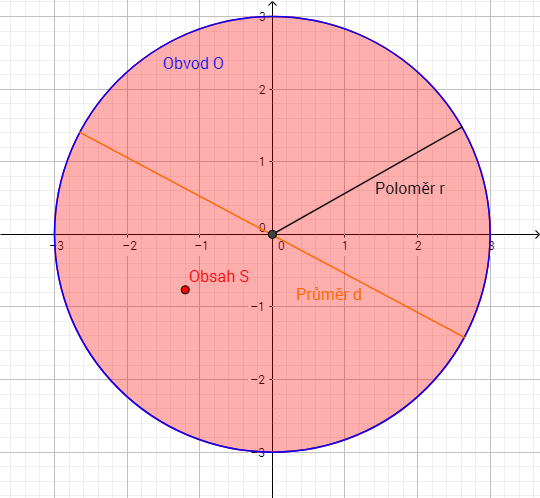
\includegraphics[width=10cm]{Circle.png}
\begin{equation}
\begin{split}
r\quad &=\quad \pi d\nonumber\\ 
d\quad &=\quad 2r\nonumber\\
O\quad &=\quad 2\pi\nonumber r\\
S\quad &=\quad \pi { r }^{ 2 }\nonumber
\end{split}
\end{equation}

\begin{multicols}{2}
\noindent
\paragraph{1.}
\begin{equation}
\begin{split}
\nonumber
r\quad &=\quad 2,5cm\\ 
O\quad &=\quad 2\pi \quad \cdot \quad 2,5\\
O\quad &=\quad 15,71cm\\ 
S\quad &=\quad \pi \quad \cdot \quad { 2,5 }^{ 2 }\\
S\quad &=\quad \pi \quad \cdot \quad 6,25\\ 
S\quad &=\quad 19,64{ cm }^{ 2 }
\end{split}
\end{equation}
\columnbreak
\paragraph{2.}
\begin{equation}
\begin{split}
\nonumber
S\quad &=\quad { 12,56cm }^{ 2 }\\
S &= \pi { r }^{ 2 }\qquad |/\pi\\
\frac { S }{ \pi  }  &= { r }^{ 2 }\qquad |\sqrt {  }  \\
\sqrt { \frac { S }{ \pi  }  }  &= r \\ 
\sqrt { \frac { 12,56 }{ \pi  }  }  &= r \\
r & = 2cm\\
d & = 2r \\ 
d & = 4cm 
\end{split}
\end{equation}
\end{multicols}

\subsection{Válec}
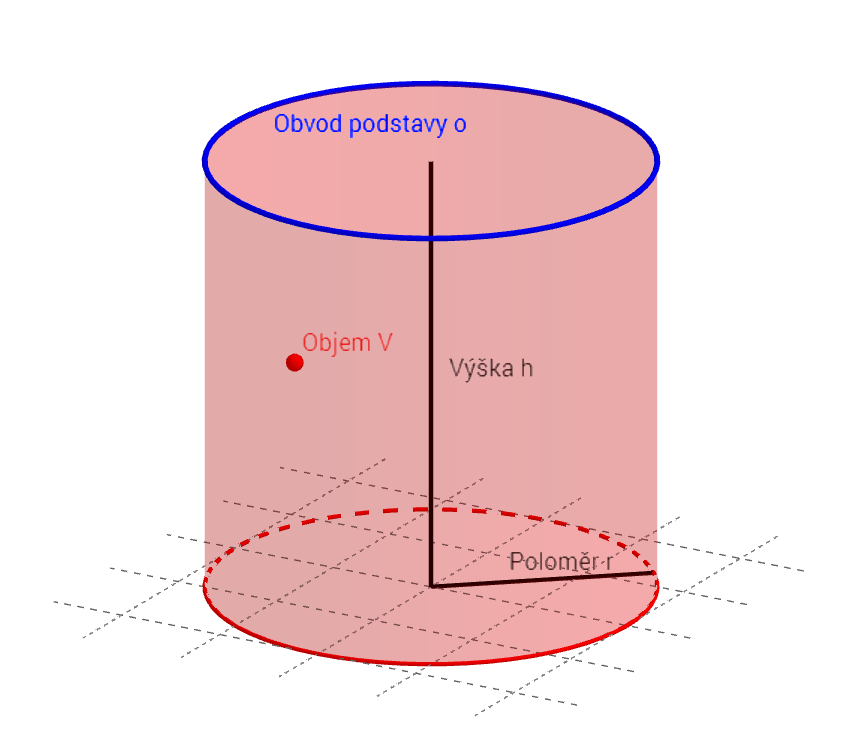
\includegraphics[width=10cm]{Cylinder.png}
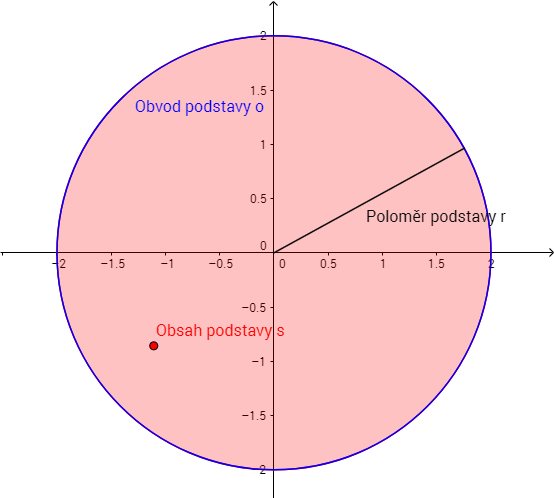
\includegraphics[width=7cm]{Cylinder_down.png}
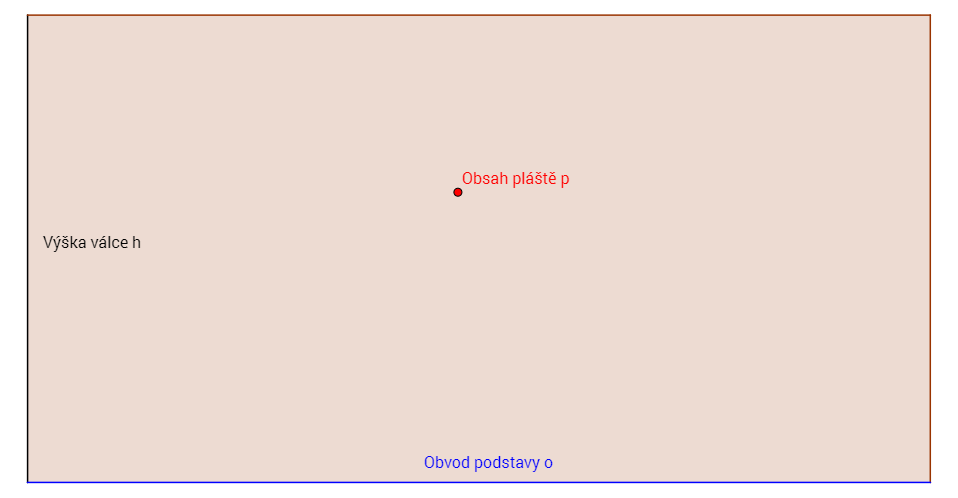
\includegraphics[width=10cm]{Cylinder_front.png}

\begin{equation}
\begin{split}
\text{Obvod podstavy }o\quad &=\quad 2\pi r\nonumber\\ 
\text{Obsah podstavy }s\quad &=\quad \pi { r }^{ 2 }\nonumber\\
\text{Obsah pláště }p\quad &=\quad oh\nonumber\\
\text{Objem válce }V\quad &=\quad sh\nonumber\\
\text{Povrch válce }P\quad &=\quad 2s+p\nonumber
\end{split}
\end{equation}

\pagebreak


\begin{multicols}{2}
\noindent
\subsubsection{Válec}
\begin{equation}
\begin{split}
\nonumber
\text{Průměr podstavy }d&=14,8dm\\
\text{Výška válce }h&=2,3m
\end{split}
\end{equation}

\begin{equation}
\begin{split}
\nonumber
\text{Poloměr podstavy }r&=\frac { 14,8dm }{ 2 }\\
r&=7,4dm=0,74m\\
\end{split}
\end{equation}

\begin{equation}
\begin{split}
\nonumber
s&=\pi { r }^{ 2 }\\
s&=\pi \cdot { 0,74 }^{ 2 }\\
s&={ 1,72m }^{ 2 }
\end{split}
\hspace{0,5cm}
\begin{split}
\nonumber
V&=s\cdot h\\
V&=1,72\cdot 2,3\\
V&={ 3,96m }^{ 3 }
\end{split}
\end{equation}
\begin{equation}
\begin{split}
\nonumber
o&=2\pi r\\
o&=2\pi \cdot 0,74\\
o&=4,65m
\end{split}
\hspace{0,5cm}
\begin{split}
\nonumber
p&=o \cdot h\\
p&=4,65 \cdot 2,3\\
p&={ 10,69m }^{ 2 }
\end{split}
\end{equation}
\begin{equation}
\begin{split}
\nonumber
P&=2s+p\\
P&=2 \cdot 1,72 + 10,69\\
P&={ 14,13m }^{ 3 }
\end{split}
\end{equation}
\subsubsection{Poloměr a výška válce}
\paragraph{1.}
\begin{equation}
\begin{split}
\nonumber
\text{Objem }V&={300cm}^{2}\\
\text{Výška }h&=8cm\\
\text{Poloměr podstavy }r&=\text{?}
\end{split}
\end{equation}
\begin{equation}
\begin{split}
\nonumber
V&=sh\\
s&=\frac{V}{h}\\
s&=\frac{300}{8}\\
s&={37,5cm}^{2}
\end{split}
\hspace{0,5cm}
\begin{split}
\nonumber
s&=\pi {r}^{2}\\
\frac{s}{\pi}&={r}^{2}\\
r&=\sqrt{\frac{s}{\pi}}\\
r&=\sqrt{\frac{37,5}{\pi}}\\
r&=3,45cm
\end{split}
\end{equation}

\paragraph{2.}
\begin{equation}
\begin{split}
\nonumber
\text{Povrch }P&={120cm}^{2}\\
\text{Poloměr podstavy }r&=2cm\\
\text{Výška válce }h&=\text{?}
\end{split}
\end{equation}
\begin{equation}
\begin{split}
\nonumber
s&=\pi { r }^{ 2 }\\
s&=\pi \cdot { 2 }^{ 2 }\\
s&={ 4cm }^{ 2 }
\end{split}
\hspace{0,5cm}
\begin{split}
\nonumber
P&=2s+p\\
p&=P-2s\\
p &= 120-2 \cdot 4\\
p &= {112cm}^{2}
\end{split}
\end{equation}

\begin{equation}
\begin{split}
\nonumber
o&=2\pi r\\
o&=2\pi \cdot 2\\
o&=12,57cm
\end{split}
\hspace{0,5cm}
\begin{split}
\nonumber
p&=oh\\
h&=\frac{p}{o}\\
h&=\frac{112}{12,57}\\
h&=8,91cm
\end{split}
\end{equation}
\end{multicols}

\pagebreak
\subsection{Konstrukční úlohy}
\subsubsection{Trojůhelník}
Sestrojte pravoúhlý trojůhelník ABC, kde c=5cm, a=4cm (užití Thaletovy kružnice)\\
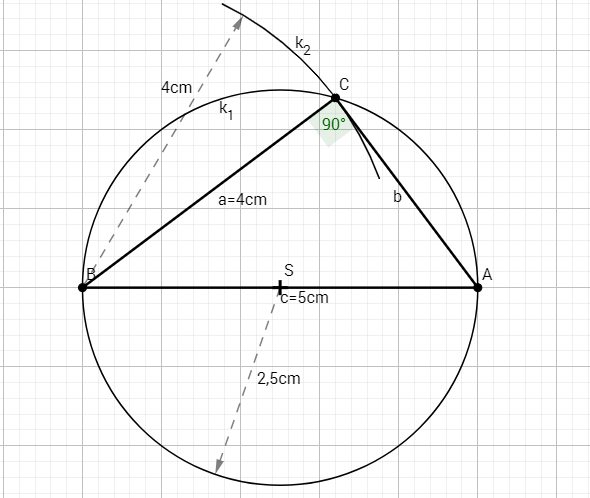
\includegraphics[width=10cm]{thalet.png}\\
Postup:
\begin{itemize}
\setlength\itemsep{1px}
\item Narýsujeme úsečku \texttt{|AB|=5cm} a nazveme ji jako stranu \texttt{c}.
\item Bod \texttt{S} nalezneme jako střed úsečky \texttt{c} (2,5cm).
\item Sestrojíme kružnici $ k_{1} $ se středem v bodě \texttt{S} a o poloměru 2,5cm (polovina strany c).
\item Sestrojíme část kružnice $ k_{2} $ se středem v bodě \texttt{B} a o poloměru 4cm (délka strany \texttt{a}).
\item Průsečík $ k_{2} $ a $ k_{1} $ označíme jako bod \texttt{C}. Spojením bodů \texttt{A, B, C} vznikne požadovaný trojůhelník.
\end{itemize}
Thaletova věta zaručuje že takto vytvořený trojůhelník bude pravoúhlý.

\subsubsection{Tečna}
Sestrojte tečnu v bodě \texttt{N}, který leží na kružnici \texttt{l} o poloměru 2cm.\\
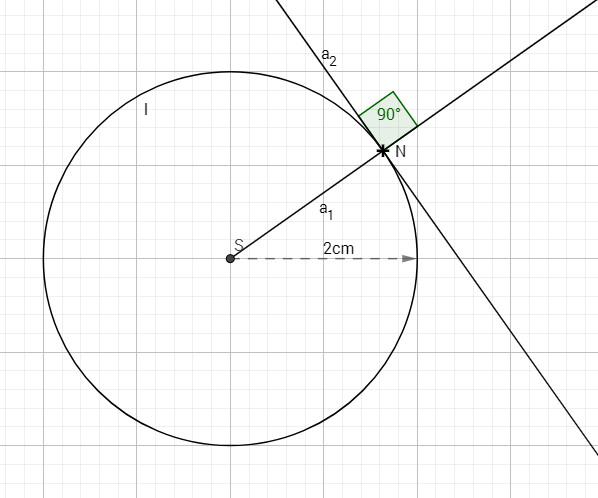
\includegraphics[width=10cm]{tangent.png}\\
Postup:
\begin{itemize}
\setlength\itemsep{1px}
\item Sestrojíme kružnici \texttt{l} o poloměru 2cm.
\item Zvolíme bod \texttt{N} ležící na kružnici.
\item Narýsujeme přímku $ a_1 $ procházející středem \texttt{S} kružnice \texttt{l} a zvoleným bodem \texttt{N}.
\item Pomocí pravítka s ryskou narýsujeme přímku $ a_2 $ kolmou na $ a_1 $ v bodě N.
\item Přímka $ a_2 $ je tečnou na kružnici \texttt{l} v bodě \texttt{N}.
\end{itemize}

\pagebreak
\section{Fyzika}
\subsection{Teplo}
Měrná tepelná kapacita \texttt{c} vody je $4180 J/Kg$ (z tabulek).
\paragraph{1.}
Voda o hmotnosti 450g zvýšila teplotu o 15$^\circ$ C. Jaké teplo přijmula?
\begin{equation}
\begin{split}
\nonumber
Q=c\cdot m\cdot (t-t_0)\\
\end{split}
\hspace{0,5cm}
\nonumber
\begin{split}
Q&\text{ ... teplo }[J]\\
c&\text{ ... měrná tepelná kapacita }[J\cdot kg^{-1}]\\
m&\text{ ... hmotnost }[Kg]\\
(t-t_0)&\text{ ... rozdíl aktuální a počáteční teploty }[^\circ C]
\end{split}
\end{equation}
\begin{equation}
\begin{split}
\nonumber
Q&=c\cdot m\cdot (t-t_0)\\
Q&=4180 \cdot 0,450 \cdot 15\\
Q&=28\, 215J\cdot kg^{-1}
\end{split}
\end{equation}

\paragraph{2.}
Bazén má délku 50m, šířku 20m a hloubka vody je 1,8m. Teplota se zvýšila z $15^\circ C$ na 25$^\circ C$. Jaké teplo voda přijmula?

Nejprve je potřeba zjistit hmotnost vody z rozměrů bazénu. Spočítáme tedy objem kvádru vody. Dále $1l=1dm^3$ a $1l$ vody váží $1Kg$.

\begin{equation}
\begin{split}
\nonumber
V&=a \cdot b \cdot c\\
V&=50\cdot 20 \cdot 1,8\\
V&=1800m^3
\end{split}
\hspace{0,5cm}
\begin{split}
\nonumber
1800m^3 &= 1800\, 000dm^3 \\
&= 1800\, 000l\\ 
&= 1800\, 000Kg\\
\end{split}
\end{equation}
\begin{equation}
\begin{split}
\nonumber
Q&=c\cdot m\cdot (t-t_0)\\
Q&=4180 \cdot 1800\, 000 \cdot (25-15)\\
Q&=75\, 240\, 000\, 000J\cdot kg^{-1}\\
Q&=75\, 240MJ\cdot kg^{-1}\\
\end{split}
\end{equation}

\pagebreak
\subsection{Zvuk}
\paragraph{3.}
Hrom následoval $18s$ po záblesku. Uvažujte rychlost šíření zvuku ve vzduchu $340m\cdot s^{-1}$. Jak daleko udeřil blesk?
\begin{equation}
\begin{split}
\nonumber
18s\cdot 340\frac{m}{s} = 6120m = 6,12Km
\end{split}
\end{equation}

\paragraph{4.}
Zvuk má frekvenci $280kHz$. Určete vlnovou délku zvuku ve vodě. Rychlost šíření zvuku ve vodě uvažujte $1500m\cdot s^{-1}$.
\begin{multicols}{2}
\noindent
\begin{equation}
\begin{split}
\nonumber
\lambda &= \frac{v}{f}\\
\end{split}
\hspace{0,5cm}
\begin{split}
\nonumber
\lambda&\text{ ... vlnová délka }[m]\\
v&\text{ ... rychlost šíření }[m\cdot s^{-1}]\\
f&\text{ ... frekvence }[Hz]\\
\end{split}
\end{equation}
\columnbreak
\noindent
\begin{equation}
\begin{split}
\nonumber
\lambda&=\frac{v}{f}\\
\lambda&=\frac{1500}{280\, 000}\\
\lambda&=0,005357m\\
\lambda&=5,36mm
\end{split}
\end{equation}
\end{multicols}
\paragraph{5.}
Signál vyslaný sonarem se vrátil odražením ode dna za $5s$ jak hluboká je voda? Rychlost zvuku ve vodě je $1500m\cdot s^{-1}$.
\begin{equation}
\begin{split}
\nonumber
\frac{1500[m\cdot s^{-1		}]\cdot 5[s]}{2} = 3750m = 3,75km
\end{split}
\end{equation}

\subsection{Elektrika}
\paragraph{1.}
Žárovka je připojená na zdroj napětí $230V$. Žárovkou protéká proud $230mA$. Urči elektrický odpor žárovky.
\begin{multicols}{2}
\begin{equation}
\begin{split}
\nonumber
U = R\cdot I
\end{split}
\hspace{0,5cm}
\begin{split}
\nonumber
U&\text{ ... napětí }[V]\\
R&\text{ ... odpor }[\Omega]\\
I&\text{ ... proud }[A]\\
\end{split}
\end{equation}
\columnbreak
\noindent
\begin{equation}
\begin{split}
\nonumber
U &= R\cdot I\\
R &=  \frac{U}{I}\\
R &=  \frac{230}{0,230}\\
R &= 1000\Omega = 1k\Omega\\
\end{split}
\end{equation}
\end{multicols}

\paragraph{2.}
Rezistorem o odporu $1250\Omega$ prochází proud $10mA$. Jaké je napětí na svorkách rezistoru?
\begin{equation}
\begin{split}
\nonumber
U &= R\cdot I\\
U &= 1250\cdot 0,010\\
U &= 12,5V
\end{split}
\end{equation}

\paragraph{3.}
Topné těleso je připojené k napětí $230V$. Odpor tělesa je $140\Omega$. Jaký proud prochází tělesem?.

\begin{equation}
\begin{split}
\nonumber
U &= R\cdot I\\
I &= \frac{U}{R}\\
I &= \frac{230}{140}\\
I &= 1,64A
\end{split}
\end{equation}

\subsubsection{Seriové a paralelní zapojení}
Sériové zapojení rezistorů:
$R_{\texttt{celkové}}=R_1+R_2$\\
Paralelní zapojení rezistorů:
$\frac{1}{R_{\texttt{celkové}}}=\frac{1}{R_1}+\frac{1}{R_2}$

\subsubsection*{1.}
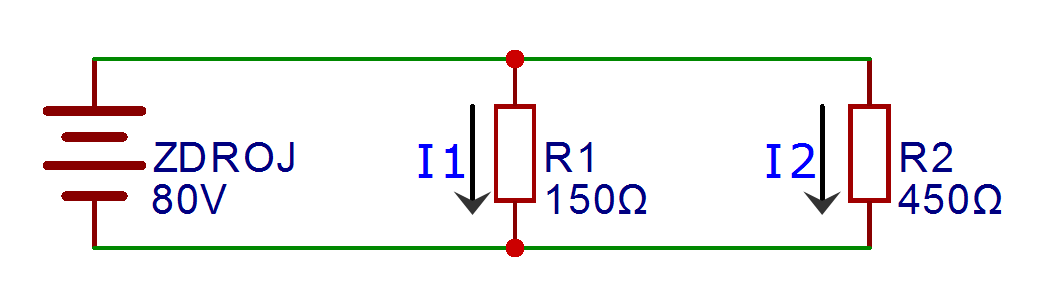
\includegraphics[width=10cm]{Ohm_001.png}
\paragraph{a)}
\begin{equation}
\begin{split}
\nonumber
\frac{1}{R_{\texttt{celkové}}}&=\frac{1}{R_1}+\frac{1}{R_2}\\
\frac{1}{R_{\texttt{celkové}}}&=\frac{1}{150}+\frac{1}{450}\\
\frac{1}{R_{\texttt{celkové}}}&=\frac{450+150}{150\cdot 450}\\
\frac{1}{R_{\texttt{celkové}}}&=\frac{450+150}{150\cdot 450}\\
\frac{1}{R_{\texttt{celkové}}}&=\frac{600}{67\, 500}\\
R_{\texttt{celkové}}&=\frac{67500}{600} = 112,5\Omega
\end{split}
\hspace{0,5cm}
\begin{split}
\nonumber
\\[4\baselineskip]
\rightarrow
\begin{cases}
\frac{1}{R_{\texttt{celkové}}}&=\frac{600}{67\, 500}\quad \rightarrow \cdot R_{\texttt{celkové}}\\
1&=\frac{600}{67\, 500}\cdot R_{\texttt{celkové}}\quad \rightarrow /\frac{600}{67\, 500}\\
\frac{1}{\frac{600}{67\, 500}}&=R_{\texttt{celkové}}\\
\frac{67\, 500}{600}&=R_{\texttt{celkové}}
\end{cases}
\end{split}
\end{equation}

\paragraph{b)}
$U_1 = U_2 = 80V$
\begin{equation}
\begin{split}
\nonumber
I_1&=\frac{U}{R_1}\\
I_1&=\frac{80}{150}\\
I_2&=0,533A = 533mA
\end{split}
\hspace{0,5cm}
\begin{split}
\nonumber
I_2&=\frac{U}{R_2}\\
I_2&=\frac{80}{450}\\
I_2&=0,177A = 177mA
\end{split}
\end{equation}
\subsubsection*{2}
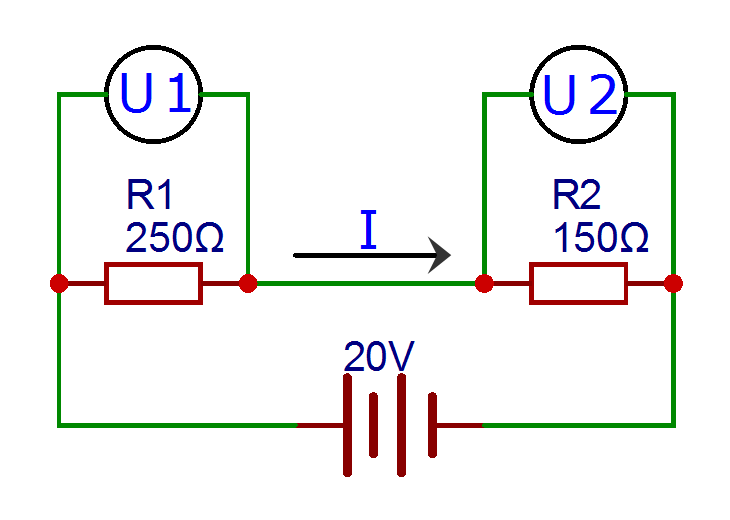
\includegraphics[width=10cm]{Ohm_002.png}
\paragraph{a)}
\begin{equation}
\begin{split}
\nonumber
R_{\texttt{celkové}}&=R_1+R_2\\
R_{\texttt{celkové}}&=250+150\\
R_{\texttt{celkové}}&=400\Omega
\end{split}
\end{equation}
\paragraph{b)}

\begin{equation}
\begin{split}
\nonumber
U_1&=R_1\cdot I\\
U_1&=250\cdot 0,05\\
U_1&=12,5V
\end{split}
\hspace{0,5cm}
\begin{split}
\nonumber
U_2&=R_2\cdot I\\
U_2&=150\cdot 0,05\\
U_2&=7,5V
\end{split}
\end{equation}
V sériovém zapojení $U_1+U_2 = U_{\texttt{celkové}}$.
\paragraph{c)}
\begin{equation}
\begin{split}
\nonumber
I&=\frac{U}{R_{\texttt{celkové}}}\\
I&=\frac{20}{400}\\
I&=0,05A = 50mA
\end{split}
\end{equation}

\subsubsection{Elektrická práce a výkon}
\begin{equation}
\begin{split}
\nonumber
P = U\cdot I
\end{split}
\hspace{0,5cm}
\begin{split}
\nonumber
P&\text{ ... příkon }[W]\\
U&\text{ ... napětí }[V]\\
I&\text{ ... proud }[A]\\
\end{split}
\hspace{0,5cm}
\begin{split}
\nonumber
W = P\cdot t
\end{split}
\hspace{0,5cm}
\begin{split}
\nonumber
W&\text{ ... elektrická práce }[Ws]\\
P&\text{ ... příkon }[W]\\
t&\text{ ... čas }[s]\\
\end{split}
\end{equation}
\begin{equation}
\begin{split}
\nonumber
Q = P\cdot t
\end{split}
\hspace{0,5cm}
\begin{split}
\nonumber
Q&\text{ ... Jouleovo teplo }[J]\\
P&\text{ ... příkon }[W]\\
t&\text{ ... čas }[s]\\
\end{split}
\end{equation}
\paragraph{1.}
Topné těleso má odpor $1,6k\Omega$ a napájí ho $12V$ baterie. Určete příkon topného tělesa a teplo které odevzdá za 2 hodiny provozu.
\begin{equation}
\begin{split}
\nonumber
I&=\frac{U}{R}\\
I&=\frac{12}{1600}\\
I&=0,0075 = 7,5mA
\end{split}
\hspace{0,5cm}
\begin{split}
\nonumber
P&=U\cdot I\\
P&=12\cdot 0,0075\\
P&=1600W
\end{split}
\end{equation}

\begin{equation}
\begin{split}
\nonumber
Q &= P\cdot t\\
Q &= 1600 \cdot (2\cdot 60)\\
Q &= 192\, 000J = 192kJ
\end{split}
\end{equation}

\paragraph{2.}
Jakou elektrickou práci vykonal proud $0,7A$ za $5h$ při napětí $230V$.
\begin{equation}
\begin{split}
\nonumber
P&=U\cdot I\\
P&=230\cdot 0,7\\
P&=161W
\end{split}
\hspace{0,5cm}
\begin{split}
\nonumber
W &= P\cdot t\\
W &= 161 \cdot (5\cdot 60)\\
W &= 48\, 300Ws = 48,3kWs
\end{split}
\hspace{0,5cm}
\begin{split}
\nonumber
1kW = 1000W\\
1h = 3600s\\
\frac{48\, 300Ws}{3\, 600\, 000}= \\
= 0,013416kWh
\end{split}
\end{equation}
\end{document}